% generated by scripts/pkl_to_latex.py
% source PKL : uscan_v1_L6_Ne6_t1_mode-uniform_nmin2_solver-gcg_sz0_restarts10_iter200_kmax4_tol1em09_U1to20_N20-d03a74da789e_vN_from_rdm_bank.pkl
% scan type  : uscan
% state      : gs
% quantity   : vn-entropy
% requires   : \usepackage{pgfplots} \pgfplotsset{compat=1.18}
% colours match the matplotlib PDF (tab10 cycle)
\definecolor{gmeC0}{HTML}{1F77B4}
\definecolor{gmeC1}{HTML}{FF7F0E}
\definecolor{gmeC2}{HTML}{2CA02C}
\definecolor{gmeC3}{HTML}{D62728}
\definecolor{gmeC4}{HTML}{9467BD}
\definecolor{gmeC5}{HTML}{8C564B}
\definecolor{gmeC6}{HTML}{E377C2}
\definecolor{gmeC7}{HTML}{17BECF}

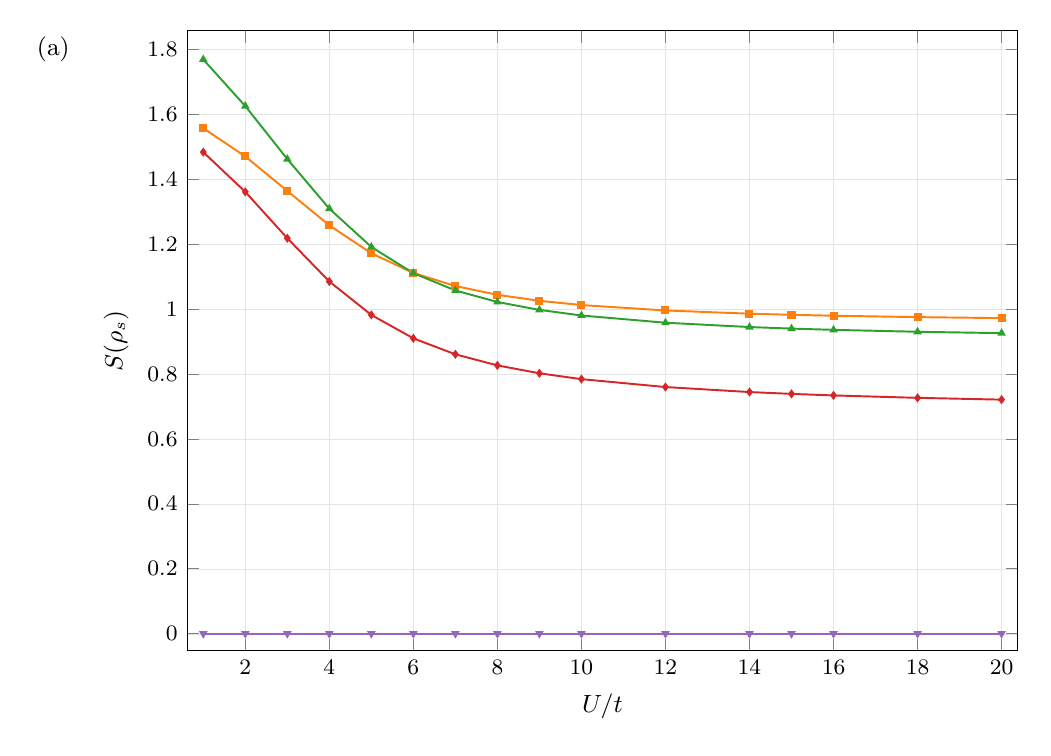
\begin{tikzpicture}
  \begin{axis}[
    width=\columnwidth,
    height=0.78\columnwidth,
    xlabel={$U/t$},
    ylabel={$S(\rho_s)$},
    grid=both,
    grid style={line width=.1pt, draw=gray!20},
    tick label style={font=\footnotesize\rmfamily, /pgf/number format/fixed},
    label style={font=\small\rmfamily},
    scaled ticks=false,
    legend style={font=\scriptsize\rmfamily, draw=gray!40, at={(0.5,1.03)}, anchor=south, /tikz/every even column/.append style={column sep=6pt}},
    legend cell align={left},
    legend columns=2,
    ymin=-0.053,
    ymax=1.857,
    xmin=0.62,
    xmax=20.38,
    after end axis/.append code={\node[anchor=east, font=\small\rmfamily] at (axis description cs:-0.13,0.970) {(a)};},
  ]
    \addplot[color=gmeC1, mark=square*, mark size=1.1pt, line width=0.7pt] coordinates {
        (1,1.556812) (2,1.469846) (3,1.363643) (4,1.257608)
        (5,1.171663) (6,1.111085) (7,1.070684) (8,1.043725)
        (9,1.02527) (10,1.012215) (12,0.995509) (14,0.985634)
        (15,0.982148) (16,0.979308) (18,0.975006) (20,0.971945)
    };
    \addplot[color=gmeC2, mark=triangle*, mark size=1.1pt, line width=0.7pt] coordinates {
        (1,1.768495) (2,1.624915) (3,1.46168) (4,1.309036)
        (5,1.191186) (6,1.110372) (7,1.057088) (8,1.02162)
        (9,0.997294) (10,0.980018) (12,0.957753) (14,0.944447)
        (15,0.939707) (16,0.935825) (18,0.929897) (20,0.925632)
    };
    \addplot[color=gmeC3, mark=diamond*, mark size=1.1pt, line width=0.7pt] coordinates {
        (1,1.483146) (2,1.360802) (3,1.217918) (4,1.08478)
        (5,0.981755) (6,0.909659) (7,0.860469) (8,0.826374)
        (9,0.802007) (10,0.784018) (12,0.759672) (14,0.744274)
        (15,0.73859) (16,0.733842) (18,0.726409) (20,0.720905)
    };
    \addplot[color=gmeC4, mark=triangle*, mark size=1.1pt, mark options={rotate=180}, line width=0.7pt] coordinates {
        (1,0) (2,0) (3,0) (4,0)
        (5,0) (6,0) (7,0) (8,0)
        (9,0) (10,0) (12,0) (14,0)
        (15,0) (16,0) (18,0) (20,0)
    };
  \end{axis}
\end{tikzpicture}
